\documentclass[]{beamer}

\usepackage[english]{babel}
\usepackage[utf8]{inputenc}
\usepackage[T1]{fontenc}
\usepackage{booktabs}
\usetheme[
  workplace=fi,
]{MU}

\graphicspath{{../}}

\newcommand{\TODO}{\textbf{\textcolor{red}{TODO}}} % red bold TODO

\begin{document}

\title[PA181]{PA181}
\subtitle[Term Project]{Term Project}

\author[A.\,Tóth, J.\,Ondruch, J.\,Čechák, T.\,Pavlík, V.\,Stehlík]{
  \begin{scriptsize}
    \begin{tabular}{r@{\hspace{2mm}}l}
      Adrián Tóth    & {\normalfont 491322@mail.muni.cz}\\[1mm]
      Jiří Čechák    & {\normalfont 445717@mail.muni.cz}\\[1mm]
      Jan Ondruch    & {\normalfont 433341@mail.muni.cz}\\[1mm]
      Tadeáš Pavlík  & {\normalfont 487555@mail.muni.cz}\\[1mm]
      Václav Stehlík & {\normalfont 487580@mail.muni.cz}\\[1mm]
    \end{tabular}
  \end{scriptsize}
}

\institute[FI MU]{Faculty of Informatics, Masaryk University}
\date{\today}
\subject{Presentation Subject}
\keywords{the, presentation, keywords}

\begin{frame}[plain]
  \maketitle
\end{frame}

\begin{frame}{Table of Contents}
  \tableofcontents
\end{frame}

%##############################################################################

\section[Introduction]{Introduction}

  \subsection{About}

    \begin{frame}{About}
      \TODO: about
    \end{frame}

  \subsection{Idea}

    \begin{frame}{Idea}
      \TODO: idea
    \end{frame}

\section[Development]{Development}

  \subsection{Work Division}

    \begin{frame}{Work Division}
      \TODO: who did what
    \end{frame}

  \subsection{Used Tools \& Technologies}

    \begin{frame}{Used Tools \& Technologies}
      \TODO: github, travis CI, ibmcloud, asp.net, react, C\#
    \end{frame}

  \subsection{Application Initialization}

    \begin{frame}{Application Initialization}
      \TODO: start, chosen template and architecture
    \end{frame}

  \subsection{Application Development}

    \begin{frame}{Application Development}
      \TODO: design and coding
    \end{frame}

  \subsection{Application Deployment}

    \begin{frame}{Application Deployment}
      \TODO
    \end{frame}

\section[Application]{Application}

  \subsection{Examples}

    \begin{frame}{Example 1}
      \begin{figure}
        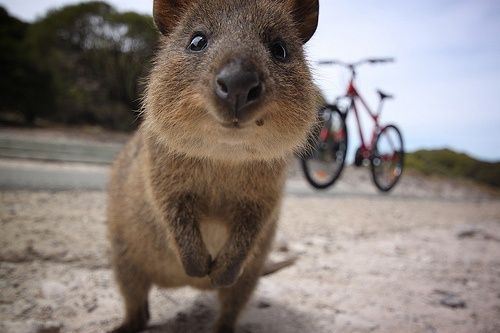
\includegraphics[width=.5\textwidth,height=.5\textheight,keepaspectratio]{img/todo.jpg}
        \caption{\TODO}
      \end{figure}
    \end{frame}

  \begin{frame}{Example 2}
      \begin{figure}
        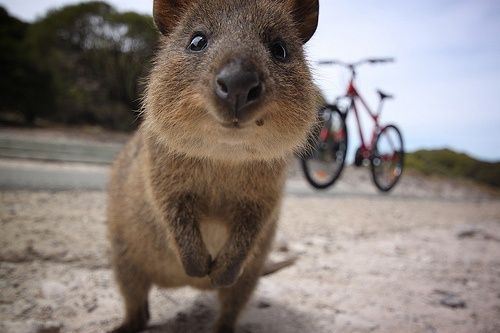
\includegraphics[width=.5\textwidth,height=.5\textheight,keepaspectratio]{img/todo.jpg}
        \caption{\TODO}
      \end{figure}
    \end{frame}

  \begin{frame}{Example 3}
      \begin{figure}
        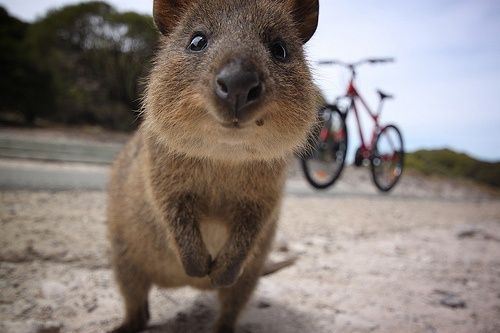
\includegraphics[width=.5\textwidth,height=.5\textheight,keepaspectratio]{img/todo.jpg}
        \caption{\TODO}
      \end{figure}
    \end{frame}

%##############################################################################

\begin{frame}[plain]
  \vspace{20mm}
  \centerline{Thank you for your attention!}
\end{frame}

\end{document}
